\documentclass{beamer}

\usepackage{amsmath}
\usepackage{amssymb}
\usepackage{amsthm}
\usepackage[UKenglish]{babel}
\usepackage{enumerate}
\usepackage{graphicx}
\usepackage{braket}
\usepackage{esint}
\usepackage{float}
\usepackage{subcaption}
\usepackage{hyperref}
\hypersetup{colorlinks=false, bookmarks=true}

\usetheme{Madrid}
\usecolortheme{seahorse}
\usefonttheme{professionalfonts}
\useinnertheme{circles}

\setbeamertemplate{caption}[numbered]

\title[PQC Function Evaluation]{PQC Function Evaluation}
\subtitle{Weeks 1-3}
\author[David Amorim]{David Amorim}
\institute[]{}
\date[22/07/2024]{01/07/2024 - 19/07/2024}

\begin{document}

\frame{\titlepage}

\begin{frame}
\frametitle{Table of Contents}
\tableofcontents
\end{frame}

\begin{frame}
\section{Background}
\frametitle{Background}

\begin{itemize}
\item Hayes 2023\footnote{\url{https://arxiv.org/pdf/2306.11073}} presents a scheme to prepare a complex vector $\boldsymbol{h} =\{ \tilde{A}_j e^{i \Psi (j)} | 0 \leq j < N \}$ as the quantum state 
\begin{equation}
\ket{h} = \frac{1}{|\tilde{A}|} \sum^{2^n-1}_{j=0} \tilde{A}(j) e^{i \Psi (j)} \ket{j}, 
\end{equation}
using $n = \lceil \log_2 N \rceil$ qubits
\item This requires operators $\hat{U}_A$ and $\hat{U}_\Psi$ such that 
\begin{align}
\hat{U}_A \ket{0}^{\otimes n} &=  \frac{1}{|\tilde{A}|} \sum^{2^n-1}_{j=0} \tilde{A}(j) \ket{j}, \\
\hat{U}_\Psi \ket{j} &= e^{i \Psi (j)} \ket{j}
\end{align}
\end{itemize}
\end{frame}

\begin{frame}
\frametitle{Background}
\begin{itemize}
\item $\hat{U}_\Psi$ is constructed via an operator $\hat{Q}_\Psi$ that performs \alert{function evaluation} in an ancilla register:
\begin{equation}
\hat{Q}_\Psi  \ket{j} \ket{0}^{\otimes m}_a = \ket{j} \ket{\Psi'(j)}_a,
\end{equation}
with $\Psi'(j) \equiv \Psi(j) / 2 \pi$
\item Currently, $\hat{Q}_\Psi$ is implemented using gate-intensive \emph{linear piecewise functions (LPFs)}
\end{itemize}
\end{frame}

\begin{frame}
\frametitle{Background}
\begin{alertblock}{Aim}
Implement $\hat{Q}_\Psi$ in a gate-efficient way using a parametrised quantum circuit (PQC)
\end{alertblock}
\vspace{1cm}
\textbf{Remark} \\
The $n$-qubit register containing the $\ket{j}$ and the $m$-qubit register containing the $\ket{\Psi'(j)}$ will be referred to as the \alert{input register} and \alert{target register}, respectively. 
\end{frame}

\begin{frame}
\section{Approach: a QCNN}
\frametitle{Approach: a QCNN}
\begin{itemize}
\item A \emph{quantum convolutional neural network} (\alert{QCNN}) is used to tackle the problem
\item A QCNN is a parametrised quantum circuit involving multiple \alert{layers}
\item Two types of network layers are implemented:
\begin{itemize}
\item \alert{Convolutional layers (CL)} involve multi-qubit entanglement gates 
\item \alert{Input layers (IL)}\footnote{Replacing the conventional QCNN \emph{pooling layers}} involve controlled single-qubit operations on target qubits 
\end{itemize}
\item Input qubits only appear as controls throughout the QCNN
\end{itemize}
\end{frame}
 
\begin{frame}
\subsection{Convolutional Layers}
\frametitle{Convolutional Layers (CLs)}
\begin{itemize}
\item Each CL involves the cascaded application of a \alert{two-qubit operator} on the target register 
\item A general two-qubit operator involves 15 parameters
\item To reduce the parameter space the canonical \alert{three-parameter operator} 
\begin{equation}
\mathcal{N}(\alpha, \beta, \gamma) = \exp \left( i \left[ \alpha X \otimes X + \beta Y \otimes Y + \gamma Z \otimes Z \right] \right)
\end{equation}
is applied, at the cost of restricting the search space 
\item This can be decomposed\footnote{\url{https://arxiv.org/pdf/quant-ph/0308006}} into 3$CX$, 3$R_z$, and 2$R_y$ gates
\item A two-parameter real version, $\mathcal{N}_\mathbb{R}(\lambda, \mu)$, can be obtained by removing the $R_z$
\end{itemize}
\end{frame} 

\begin{frame}
\frametitle{Convolutional Layers (CLs)}
\begin{itemize}
\item Two types of convolutional layers are implemented:\footnote{Loosely based on Sim 2019 (\url{https://arxiv.org/pdf/1905.10876})}
\begin{itemize}
\item \alert{Neighbour-to-neighbour / linear CLs}: the $\mathcal{N}$ (or $\mathcal{N}_\mathbb{R}$) gate is applied to neighbouring target qubits 
\item \alert{All-to-all /quadratic CLs}: the $\mathcal{N}$ (or $\mathcal{N}_\mathbb{R}$) gate is applied to all combinations of target qubits
\end{itemize}
\item The $\mathcal{N}$-gate cost of neighbour-to-neighbour (NN) layers is \alert{$\mathcal{O}(m)$} while that of all-to-all (AA) layers is \alert{$\mathcal{O}(m^2)$}
\item The QCNN uses alternating linear and quadratic CLs
\end{itemize}
\end{frame} 

\begin{frame}
\subsection{Input Layers}
\frametitle{Input Layers (ILs)}
\begin{itemize}
\item ILs, replacing pooling layers, feed information about the input register into the target register 
\item An IL involves a sequence of controlled generic single-qubit rotations (\alert{$CU3$ gates}) on the target qubits, with input qubits as controls
\item For an IL producing states with \alert{real} amplitudes, the $CU3$ gates are replaced with \alert{$CR_y$ gates}
\item Each input qubit controls precisely one $CU3$ (or $CR_y$ operation), resulting in an \alert{$\mathcal{O}(n)$} gate cost (no CX gates!)
\item ILs are inserted after every second convolutional layer, alternating between control states 0 and 1  
\end{itemize}
\end{frame}

\begin{frame}
\subsection{Summary: QCNN Structure}
\frametitle{Summary: QCNN Structure}
\begin{figure}[h]
\centering
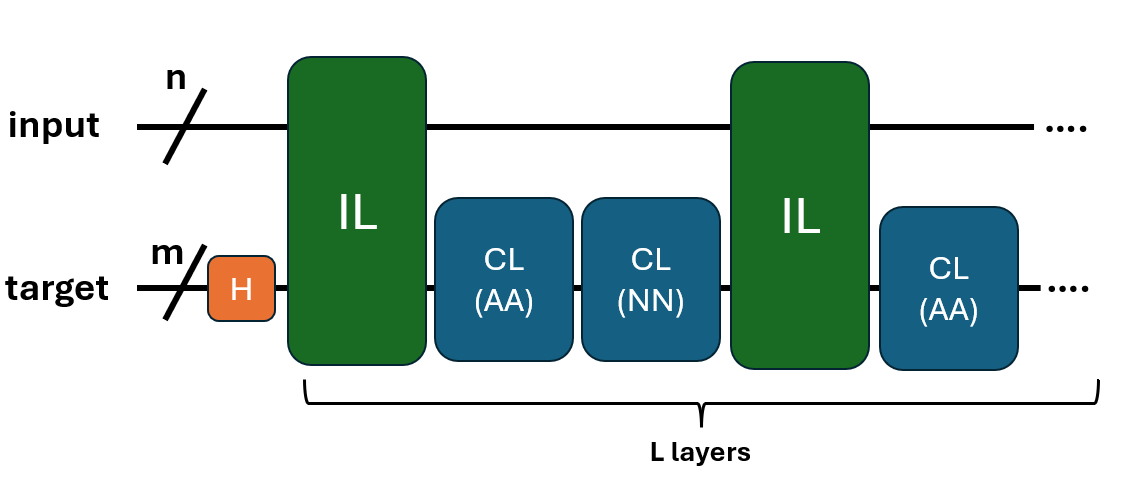
\includegraphics[width=\linewidth]{im/QCNN_structure}
\caption{Schematic of QCNN structure}
\end{figure}
\end{frame}

\begin{frame}
\section{Training the QCNN}
\frametitle{Training the QCNN}
\begin{itemize}
\item For training, the QCNN is wrapped as a \emph{SamplerQNN} object and connected to PyTorch's \alert{Adam optimiser} via \emph{TorchConnector}
\item The optimiser determines improved parameter values for each training run (\alert{epoch}) based on the \alert{loss} between output and target state
\item Beyond loss, \alert{mismatch} is an important metric:
\begin{equation}
\mathsf{M}= 1 - |\braket{\psi_\text{target}| \psi_\text{out}}|
\end{equation}
\item There are two ways to train the QCNN on input data:\footnote{One can also train the QCNN to produce a target distribution independent of the input register, which is equivalent to constructing $\hat{U}_A$}
\begin{enumerate}
\item Training on \alert{individual states}
\item Training in \alert{superposition}
\end{enumerate}
\end{itemize}
\end{frame}

\begin{frame}
\frametitle{Training the QCNN}
\begin{block}{1. Training on Individual States}
\begin{itemize}
\item One of the $2^n$ input states, $\ket{j},$ is \alert{randomly chosen} each epoch
\item The network is taught to transform $\ket{j}\ket{0} \mapsto \ket{j}\ket{\Psi'(j)} $ for each of the states individually
\end{itemize} 
\end{block}
%\vspace{1cm}
\begin{block}{2. Training in Superposition}
\begin{itemize}
\item The \alert{same input state} is chosen each epoch
\item The network is taught to transform 
\begin{equation}
\left(\frac{1}{\sqrt{2^n}} \sum^{2^n-1}_{j=0} \ket{j} \right) \ket{0} \mapsto \frac{1}{\sqrt{2^n}} \sum^{2^n -1}_{j=0} \ket{j}\ket{\Psi'(j)}
\end{equation}
\item By linearity, this teaches the network to transform $\ket{j}\ket{0} \mapsto \ket{j}\ket{\Psi'(j)} $ for each $\ket{j}$
\end{itemize} 
\end{block}
\end{frame}

\begin{frame}
\section{Initial Tests}
\frametitle{Initial Tests}
\begin{itemize}
\item Initial tests need to be carried out to \alert{inform QCNN design choices} regarding:
\begin{enumerate}[(a)]
\item Number of layers
\item Number of epochs 
\item Training mode (individually versus in superposition)
\item Use of $\mathcal{N}$ and $CU3$ versus $\mathcal{N}_\mathbb{R}$ and $CR_y$ 
\item Choice of loss function
\item Network structure
\end{enumerate}
\item This constitutes a \alert{large parameter space} that is difficult to explore systematically
\item Overly simple benchmark problems (e.g.
$n=m=2$, $\Psi(x)=x$) do not extrapolate well to more general cases 
\item Thus, tests are carried out for simplified versions of $\Psi$ in the context of Hayes 2023 ($n=6$, $m \geq 3$)
\end{itemize}
\end{frame}

\begin{frame}
\frametitle{Initial Tests}
\begin{columns}
\begin{column}{0.5\textwidth}
\begin{itemize}
\item \alert{Heuristically}: train in superposition with real circuits ($\mathcal{N}_\mathbb{R}$ and $CR_y$) of depth $L =6$ using 600 epochs and \alert{focus} on optimising the \alert{loss function}
\item Best results achieved with \emph{cross entropy} (\alert{CE}) and \emph{sign-adjusted mismatch} (\alert{SAM}):
\begin{equation}
\mathsf{SAM}(x,y) = \left\vert 1 - \sum_j x_j y_j \right \vert 
\end{equation}
\item SAM is tailored to reduce mismatch and enforce positive amplitudes
\end{itemize}
\end{column}
\begin{column}{0.5\textwidth}
\begin{figure}[h]
\centering
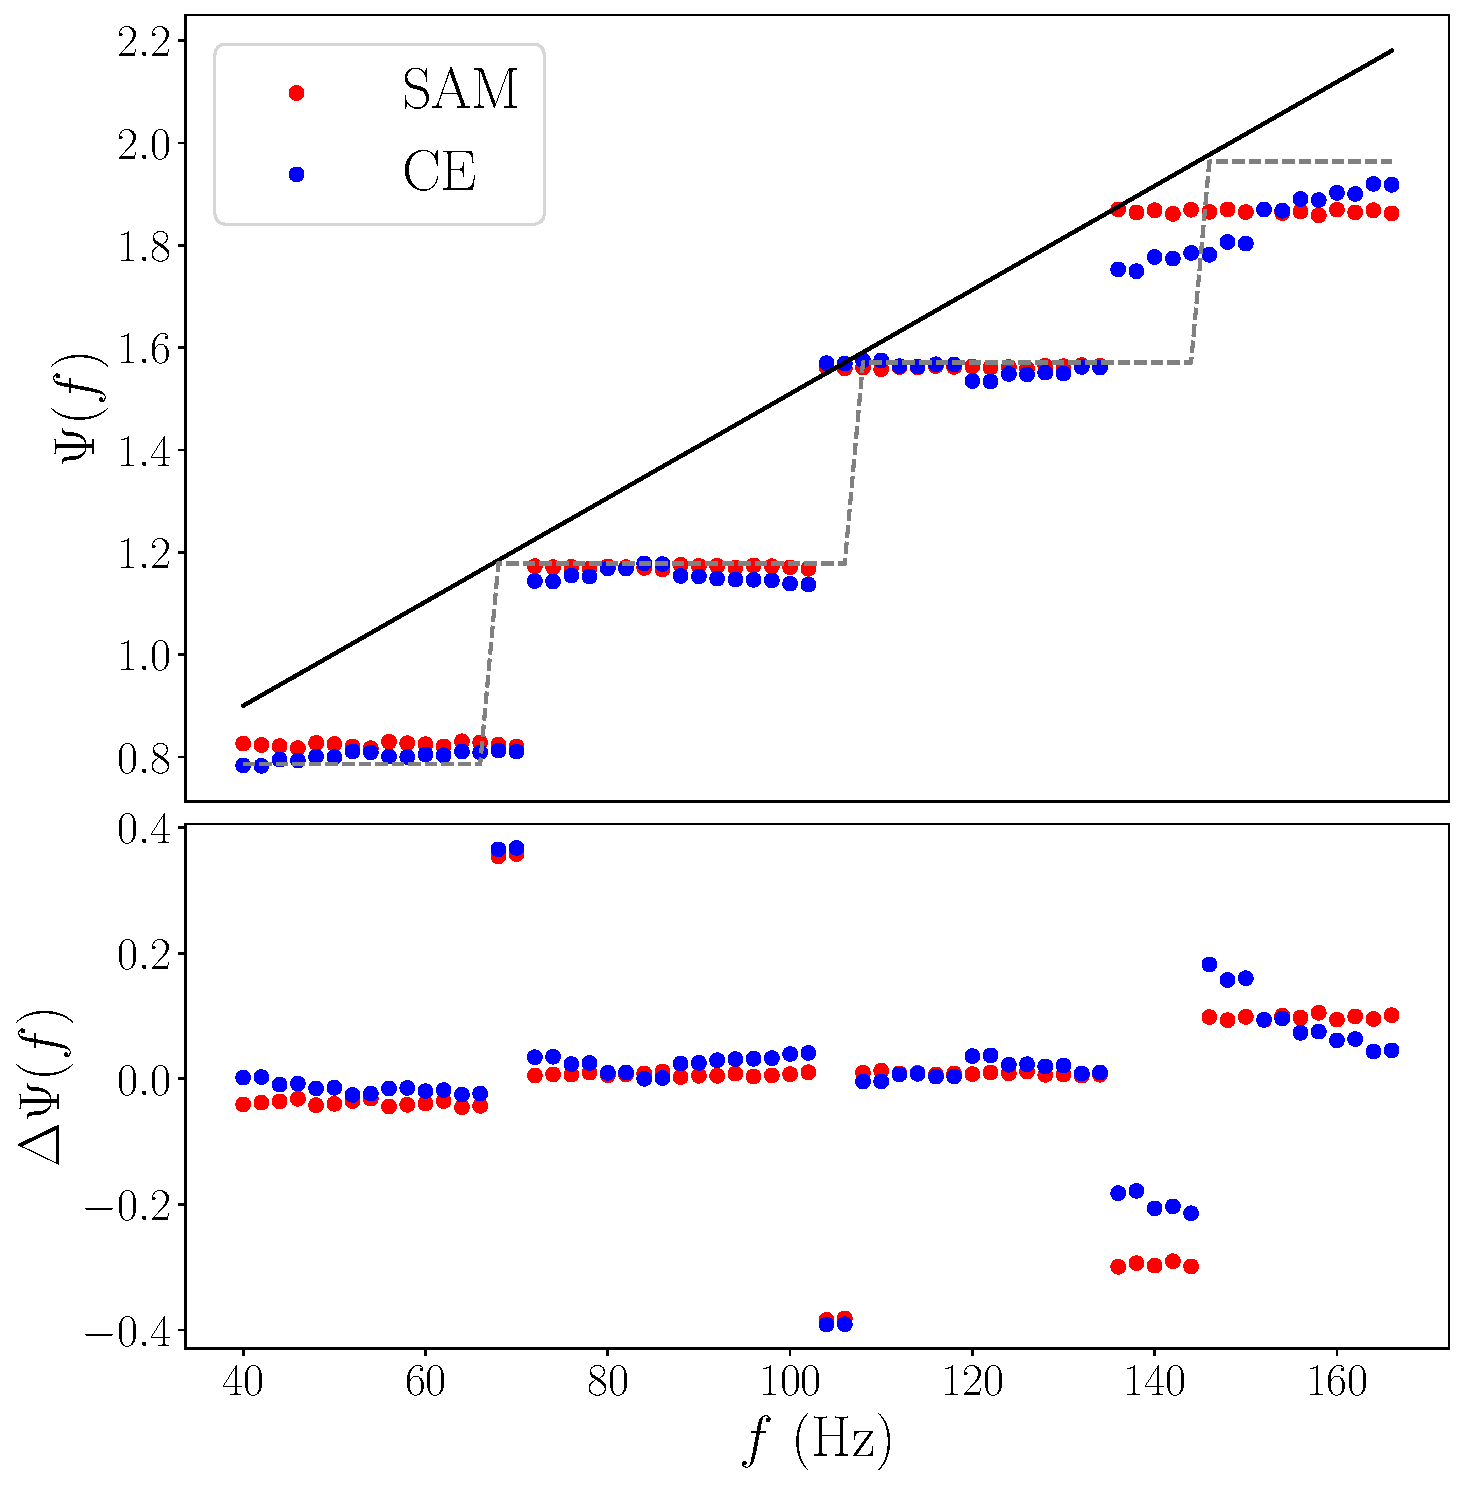
\includegraphics[width=\textwidth]{im/phase_loss_comp_linear_m4}
\caption{Comparison of loss functions for $\Psi \sim x$ and $m=4$. Target in black; rounded target dashed in grey.}
\end{figure}
\end{column}
\end{columns}
\end{frame}

\begin{frame}
\frametitle{Initial Tests}
\begin{columns}
\begin{column}{0.5\textwidth}
\begin{figure}[h]
\centering
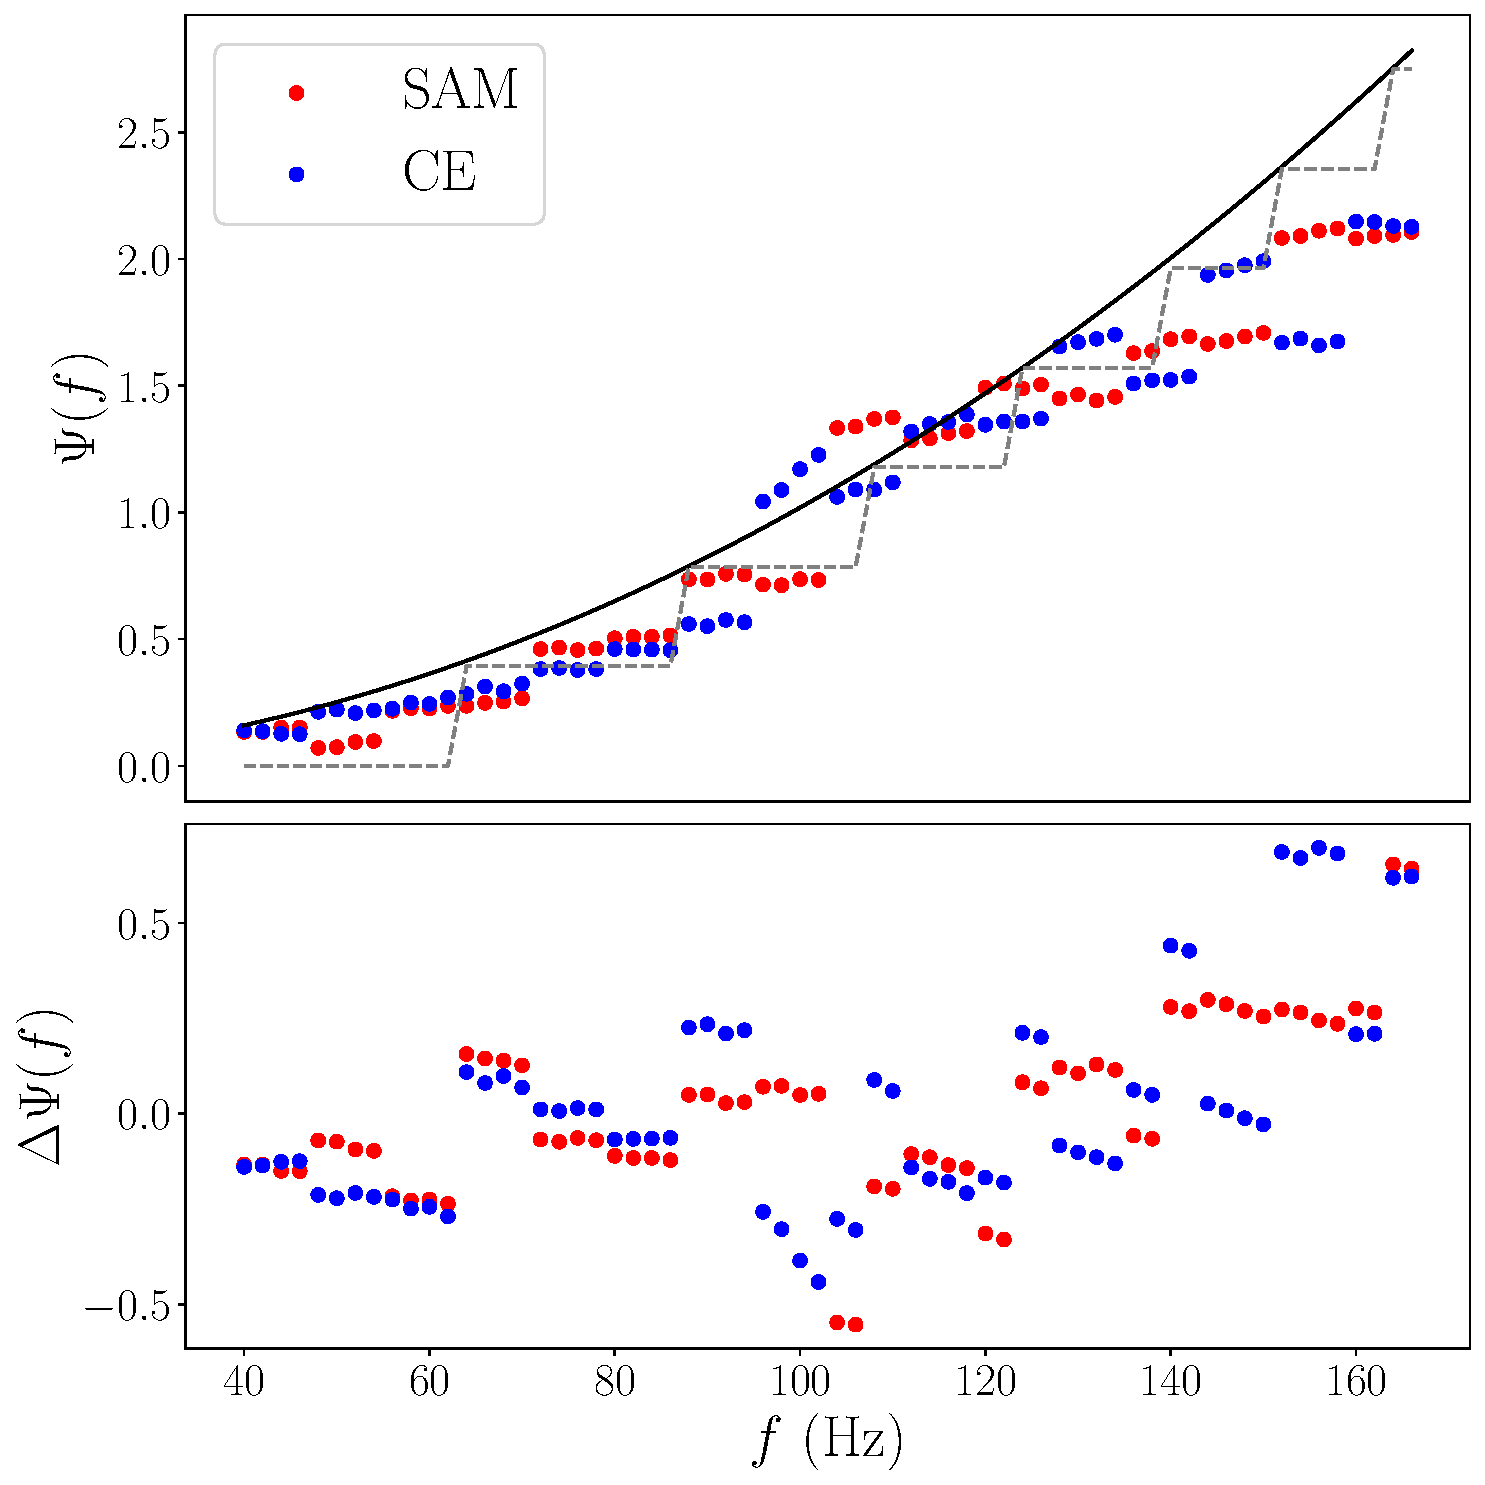
\includegraphics[width=\textwidth]{im/phase_loss_comp_quadratic_m4}
\caption{Comparison of loss functions for $\Psi \sim x^2$ and $m=4$. Target in black; rounded target dashed in grey.}
\end{figure}
\end{column}
\begin{column}{0.5\textwidth}
\begin{figure}[h]
\centering
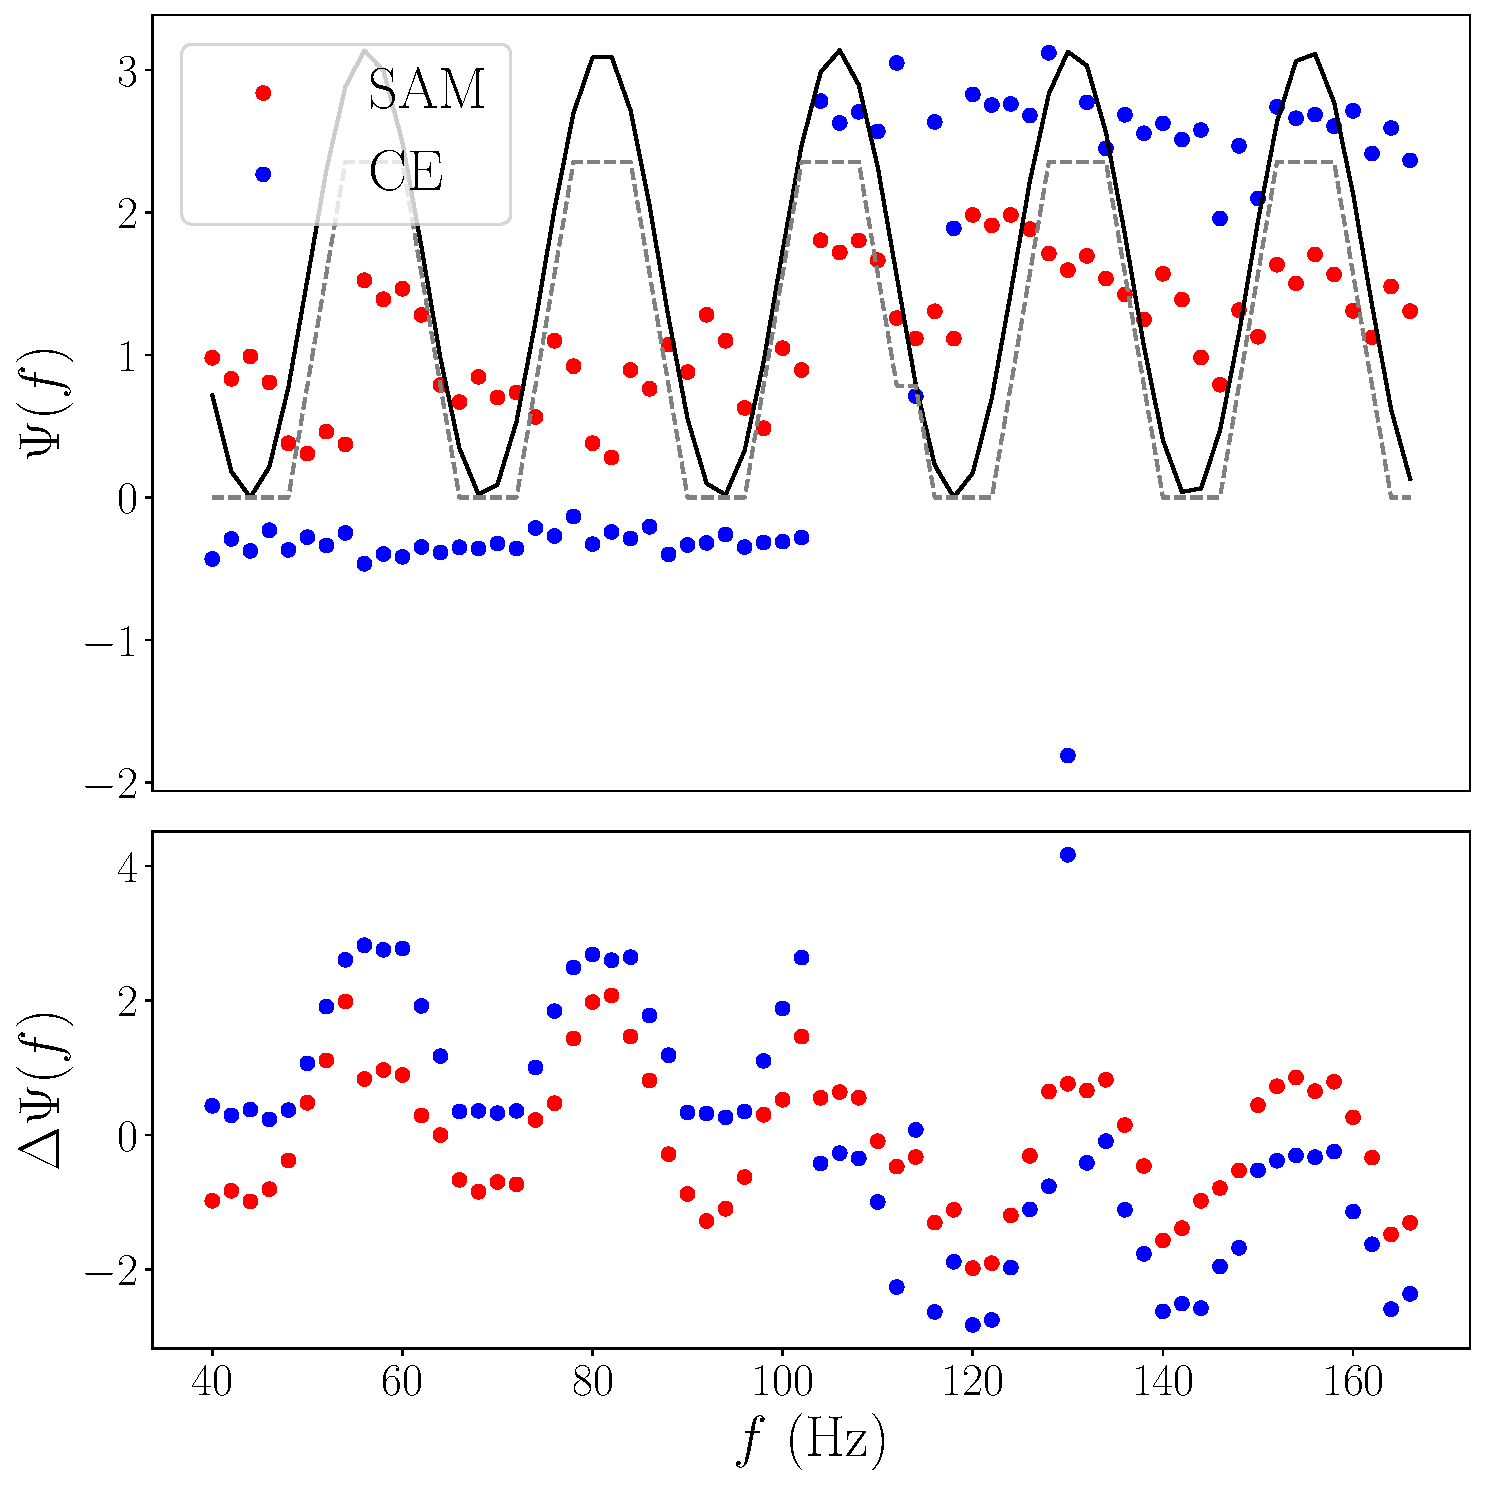
\includegraphics[width=\textwidth]{im/phase_loss_comp_sin_m3}
\caption{Comparison of loss functions for $\Psi \sim \sin x$ and $m=3$. Target in black; rounded target dashed in grey.}
\end{figure}
\end{column}
\end{columns}
\end{frame}

\begin{frame}
\frametitle{Initial Tests}
\begin{itemize}
\item \alert{SAM} significantly \alert{outperforms CE} when taking into account state amplitudes 
\item QCNN performance not much improved by increasing $L$ or number of epochs\footnote{Based on just a few tests} (\alert{no brute force solution})
\item Instead implement a \alert{weighted loss function}, taking into account the features of $\Psi$: define \emph{weighted mismatch} (\alert{WIM}) as 
\begin{equation}
\mathsf{WIM}(x,y) =  \left\vert 1 - \sum_j w_j x_j y_j \right \vert, 
\end{equation}
where the weights $w_n \in \mathbb{R}_{+}$ may be recomputed between epochs
\item When training in superposition take $w_j$ to be the (normalised) mismatch between $\hat{Q}_\Psi \ket{j} \ket{0}$ and $\ket{j}\ket{\Psi'(j)}$

\end{itemize}
OR maybe base weighting on size of "plateau" ? (need to normalise $w x$!) ; or maybe on gradient ??
\end{frame}

\begin{frame}
\section{Results}
\frametitle{Results}
\begin{itemize}
\item In the following, a QCNN is applied to implement both $\hat{U}_A$ and $\hat{U}_\Psi$ for the problem studied in Hayes 2023:
\begin{align}
\tilde{A}(f) &= f^{-7/6}, \\
\Psi(f) &= c_0 + c_1 f + c_2 f^{-1/3} + c_3 f^{-2/3} + c_4 f^{-1} + c_5 f^{-5/3},
\end{align}
with 40$\,$Hz $\leq f \leq $ 168$\,$Hz
\item In the paper, $\hat{U}_A$ is implemented via a quantum generative adversarial network (\alert{QGAN}) as well as the Grover-Rudolph (\alert{GR}) algorithm while \alert{LPFs} are used for $\hat{U}_\Psi$
\item Hayes 2023 uses $n=6$ as well as 22 ancilla qubits 
\end{itemize}
\end{frame}

\begin{frame}
\subsection{Encoding the Amplitude}
\frametitle{Encoding the Amplitude}
\begin{columns}
\begin{column}{0.5\textwidth}
\begin{itemize}
\item The \alert{QCNN outperforms the QGAN} and \alert{nearly reaches GR} w.r.t. mismatch 
\item The QCNN ($L=3$, $n=6$) was trained in 600 epochs with SAM
\end{itemize}
\vspace{0.4cm}
\begin{table}
\centering 
\begin{tabular}{c| c| c}
\textbf{Method} & \textbf{CX} & \textbf{Mismatch}  \\ \hline  
QGAN & 100 & $8.6\times10^{-3}$   \\
GR\footnote[frame]{Hayes 2023 reports a mismatch of $4.1\times 10^{-4}$} & 23,796 & $5.7\times10^{-4}$ $\,$  \\
QCNN  & 72 & $7.1\times10^{-4}$
\end{tabular}
\caption{Comparison of $\hat{U}_A$ implementations}
\end{table}
\end{column}
\begin{column}{0.5\textwidth} 
\begin{figure}[h]
\centering
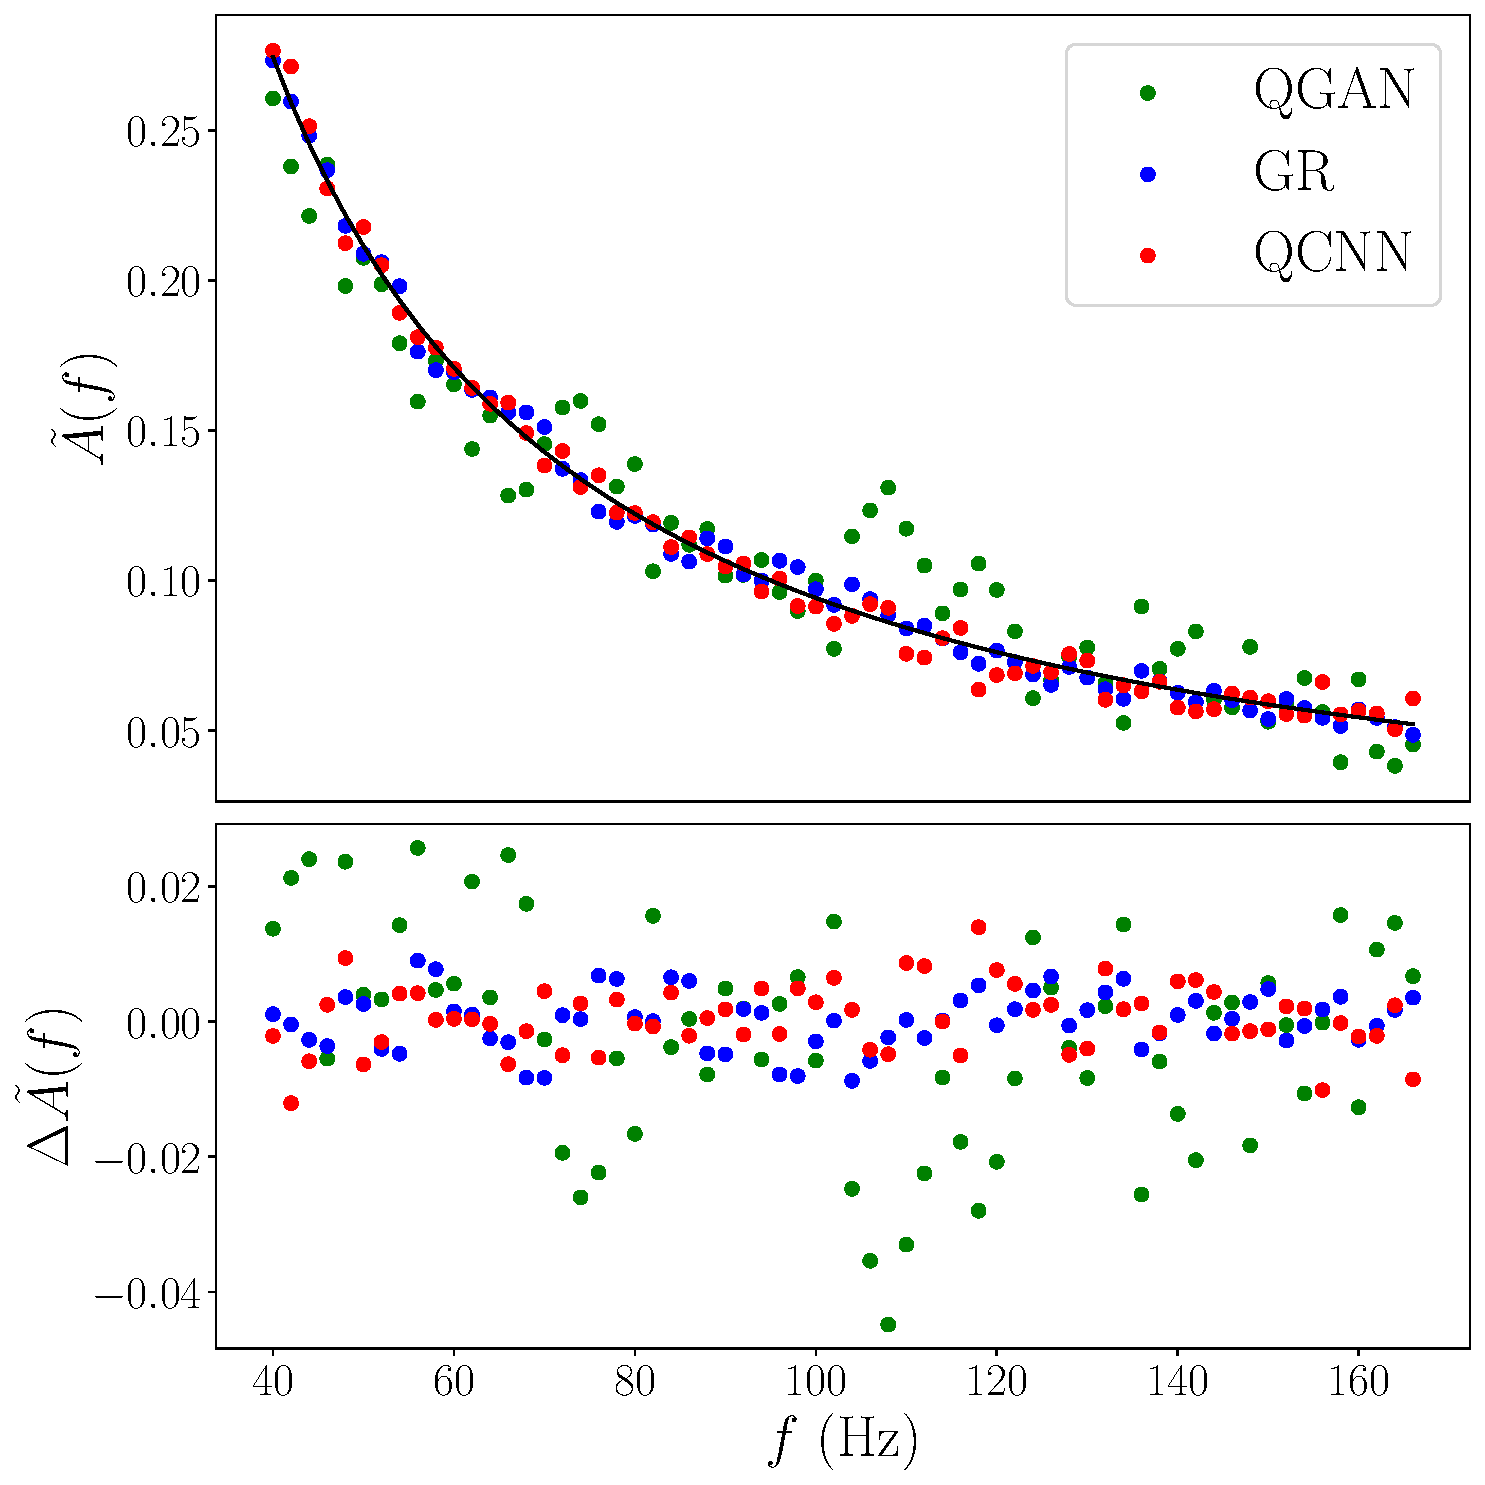
\includegraphics[width=\textwidth]{im/amplitude_comp}
\caption{Reconstruction of $\tilde{A}(f)$ from different methods. Target in black.}
\end{figure}
\end{column}
\end{columns}
\end{frame}

\begin{frame}
\frametitle{Encoding the Amplitude}
\begin{columns}
\begin{column}{0.5\textwidth}
\begin{figure}[h]
\centering
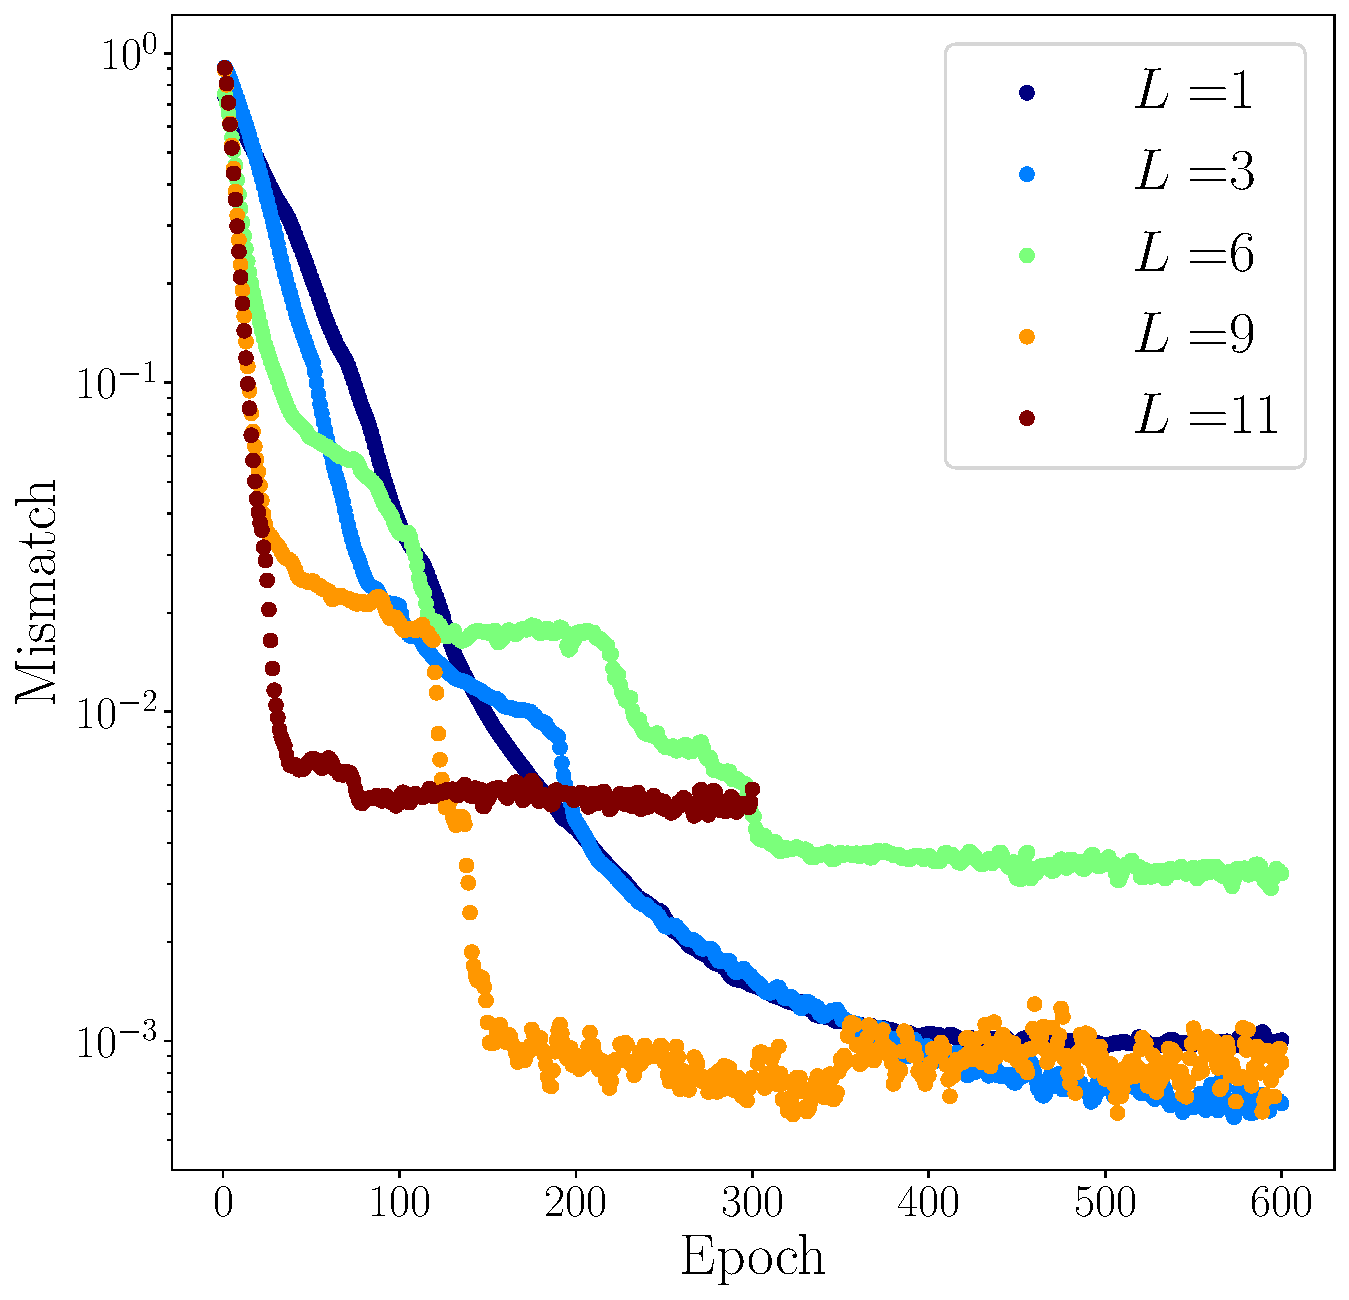
\includegraphics[width=\textwidth]{im/A_L_comp}
\caption{QCNN training for different circuit depths.}
\end{figure}
\end{column}
\begin{column}{0.5\textwidth}  
\begin{figure}[h]
\centering
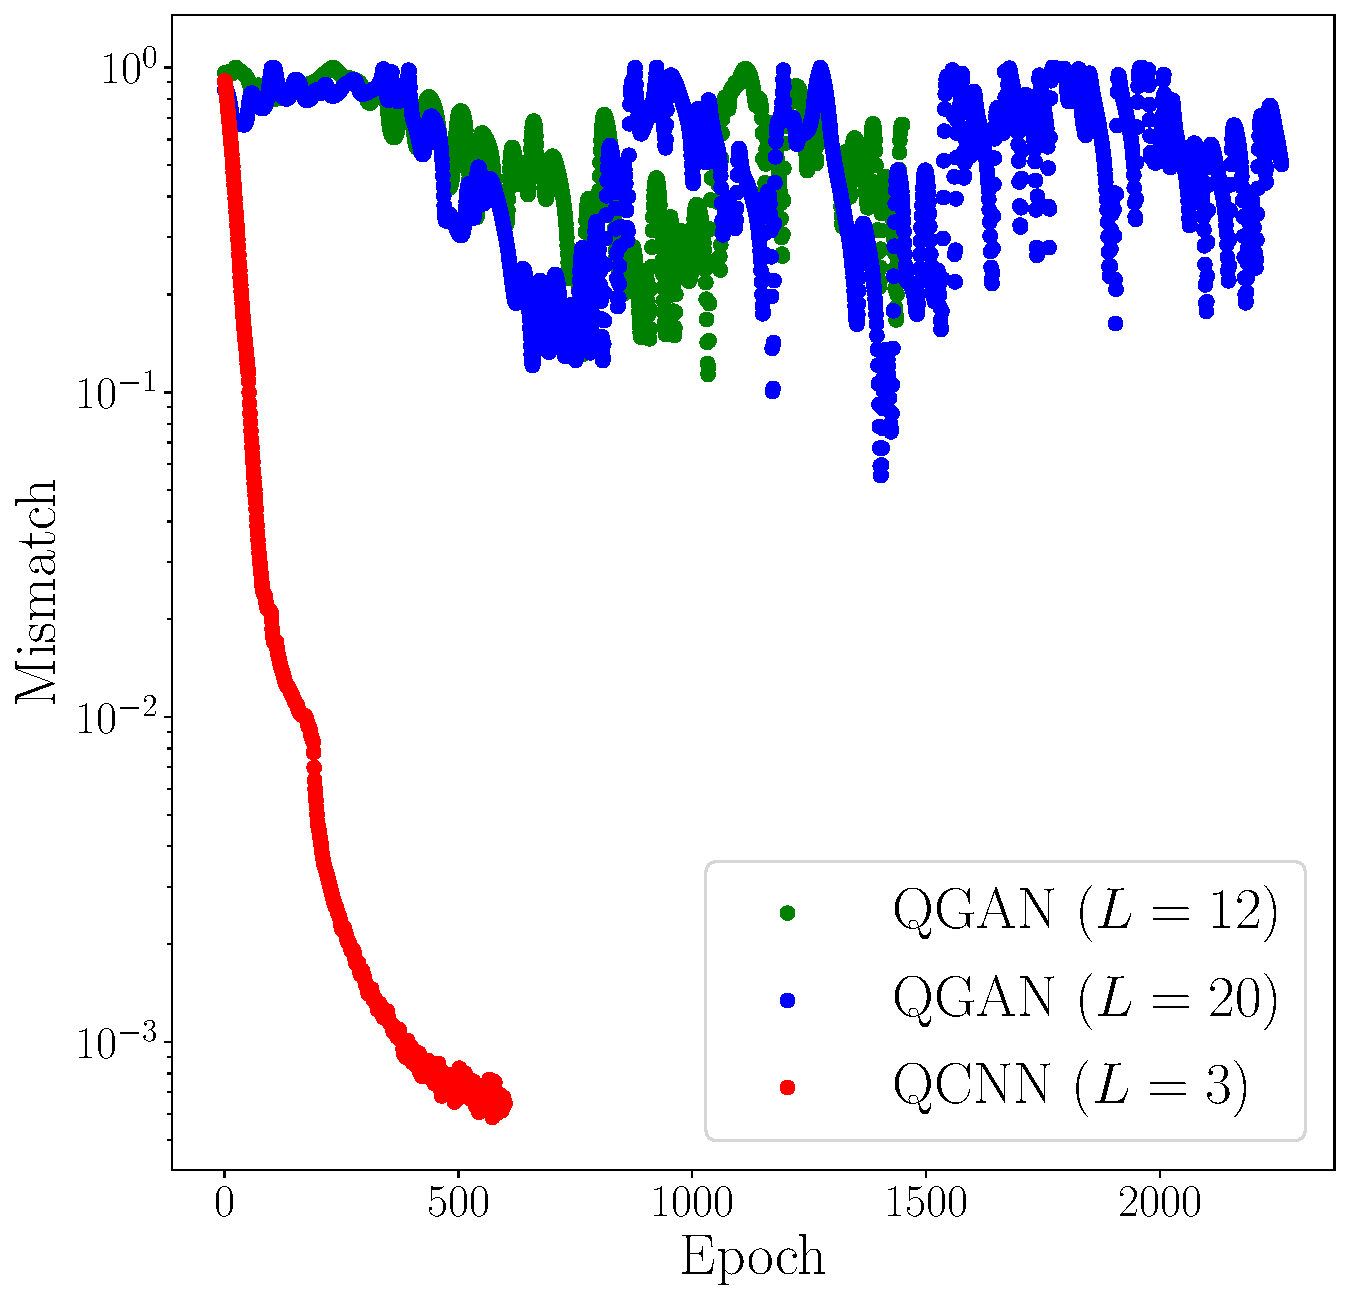
\includegraphics[width=\textwidth]{im/QGAN_comp}
\caption{Comparison of QGAN and QCNN training. Note: QGAN results do not match Hayes 2023!}
\end{figure}
\end{column}
\end{columns}
\end{frame}

\begin{frame}
\subsection{Encoding the Phase}
\frametitle{Encoding the Phase}
\begin{columns}
\begin{column}{0.5\textwidth}
\begin{itemize}
\item The implementation of $\hat{U}_\Psi$ is not the only factor affecting the encoding of $\Psi(f)$
\item The size, $m$, of the target register limits the available precision due to rounding to $\sim 2^{-m}$ 
\item A meaningful representation of $\Psi(f)$  requires $m \gtrsim 6$
\item The LPF approach in Hayes 2023 uses $m=8$
\end{itemize}
\end{column}
\begin{column}{0.5\textwidth}  
\begin{figure}[h]
\centering
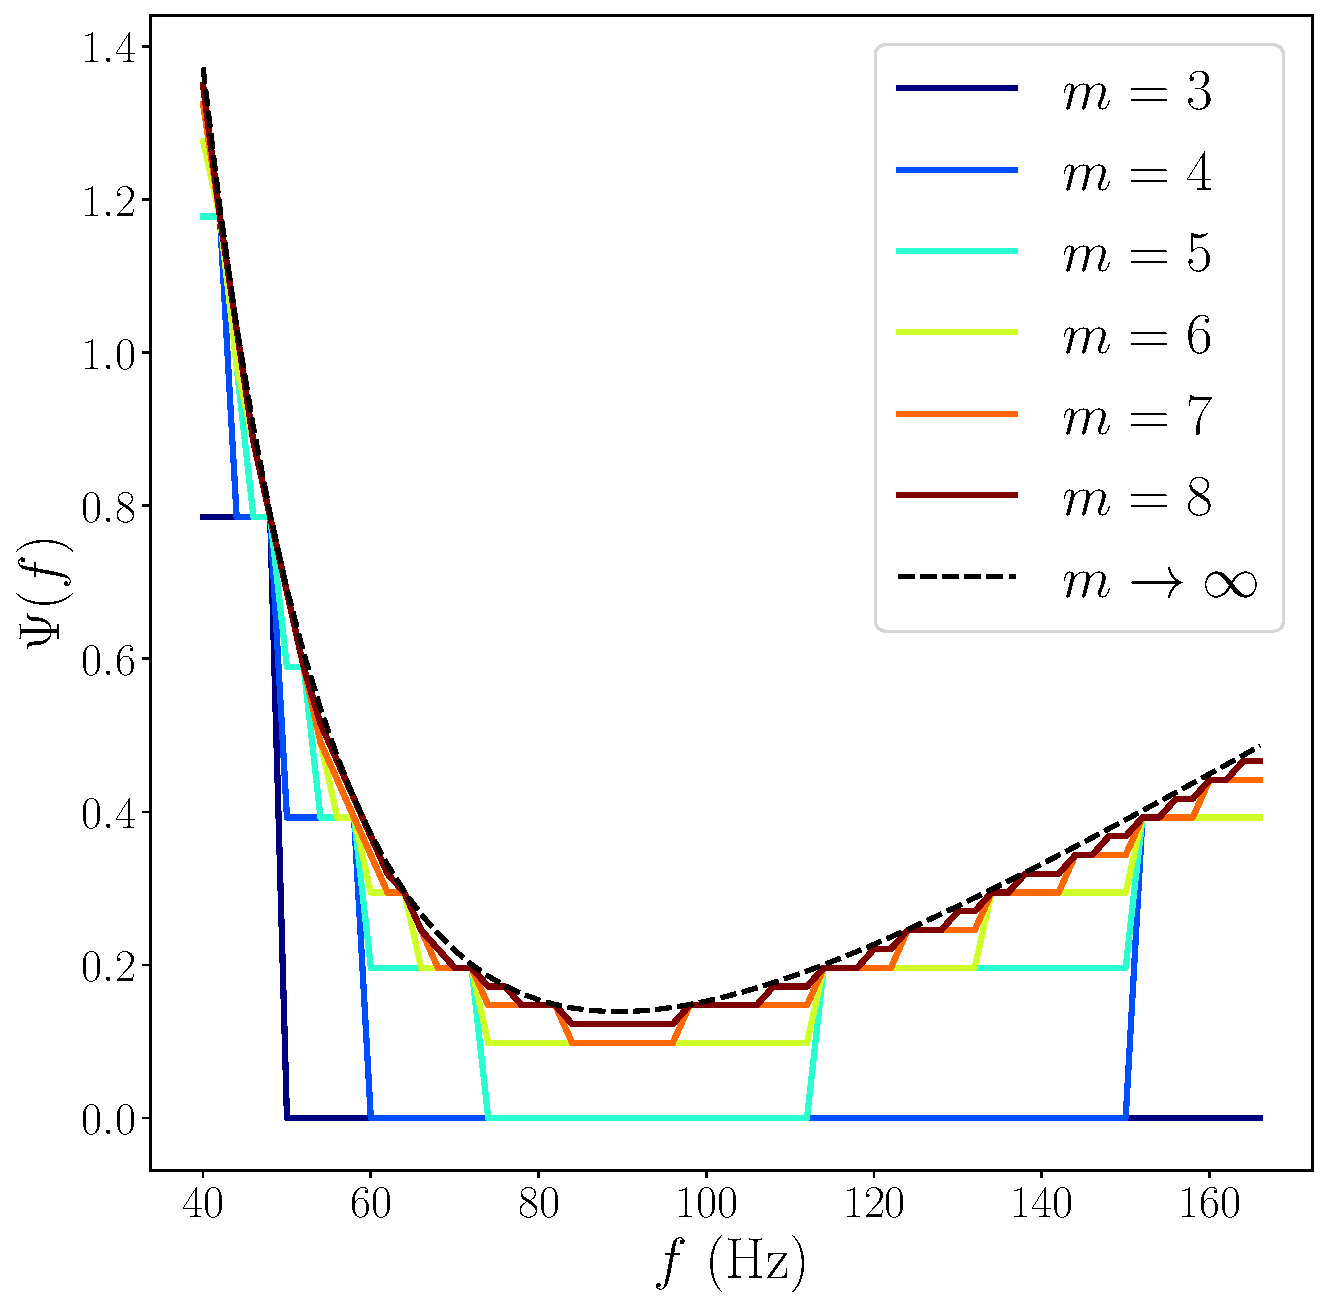
\includegraphics[width=\textwidth]{im/phase_round_comp}
\caption{Attainable precision due to rounding for different target register sizes}
\end{figure}
\end{column}
\end{columns}
\end{frame}

\begin{frame}
\frametitle{Encoding the Phase}
\begin{columns}
\begin{column}{0.5\textwidth}
\begin{itemize}
\item ...
\end{itemize}
\end{column}
\begin{column}{0.5\textwidth}  
\begin{figure}[h]
\centering
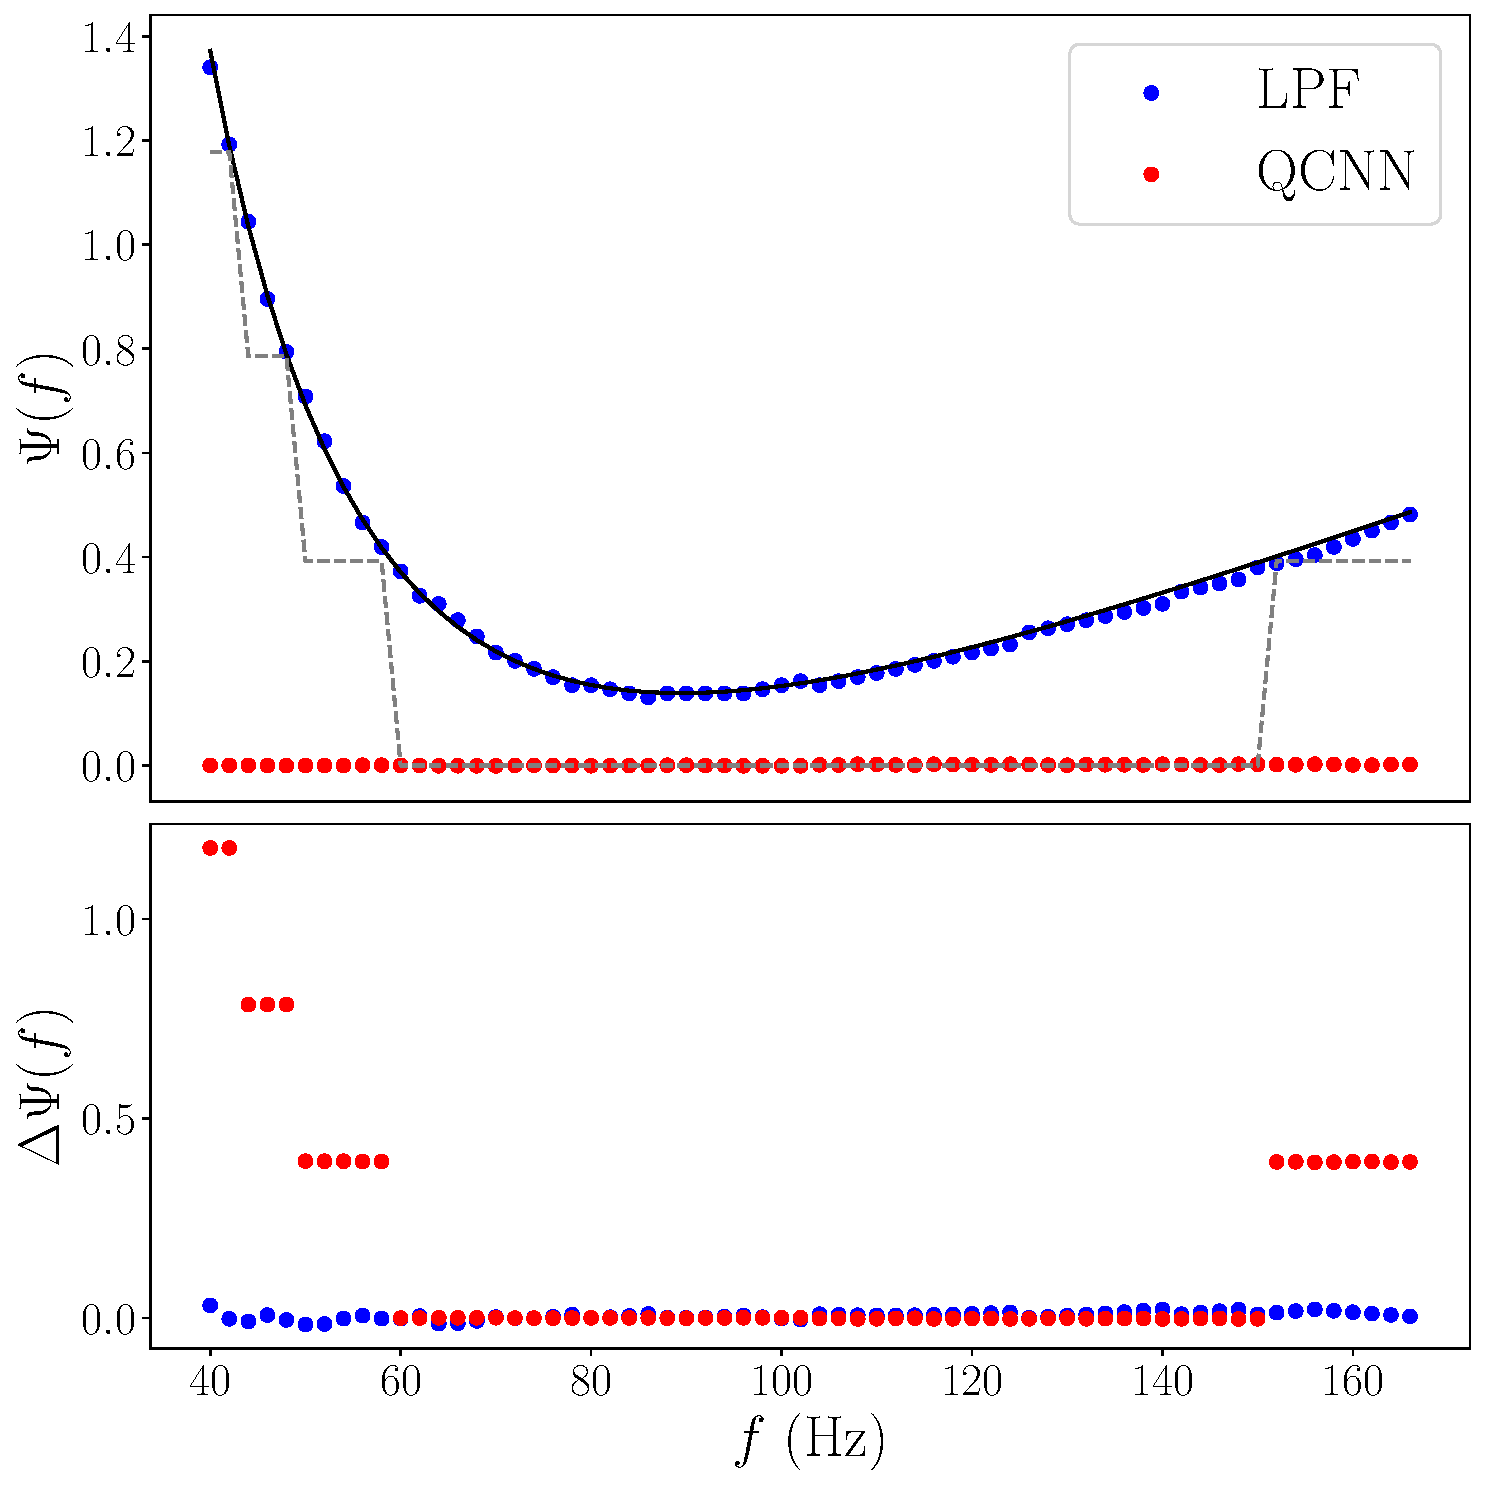
\includegraphics[width=\textwidth]{im/phase_comp}
\caption{Encoding of $\Psi(f)$ using LPFs versus a QCNN. Target in black; rounded target dashed in grey.}
\end{figure}
\end{column}
\end{columns}
\end{frame}

\begin{frame}
\subsection{Full Waveform}
\frametitle{Full Waveform}
\begin{figure}[h]
\centering
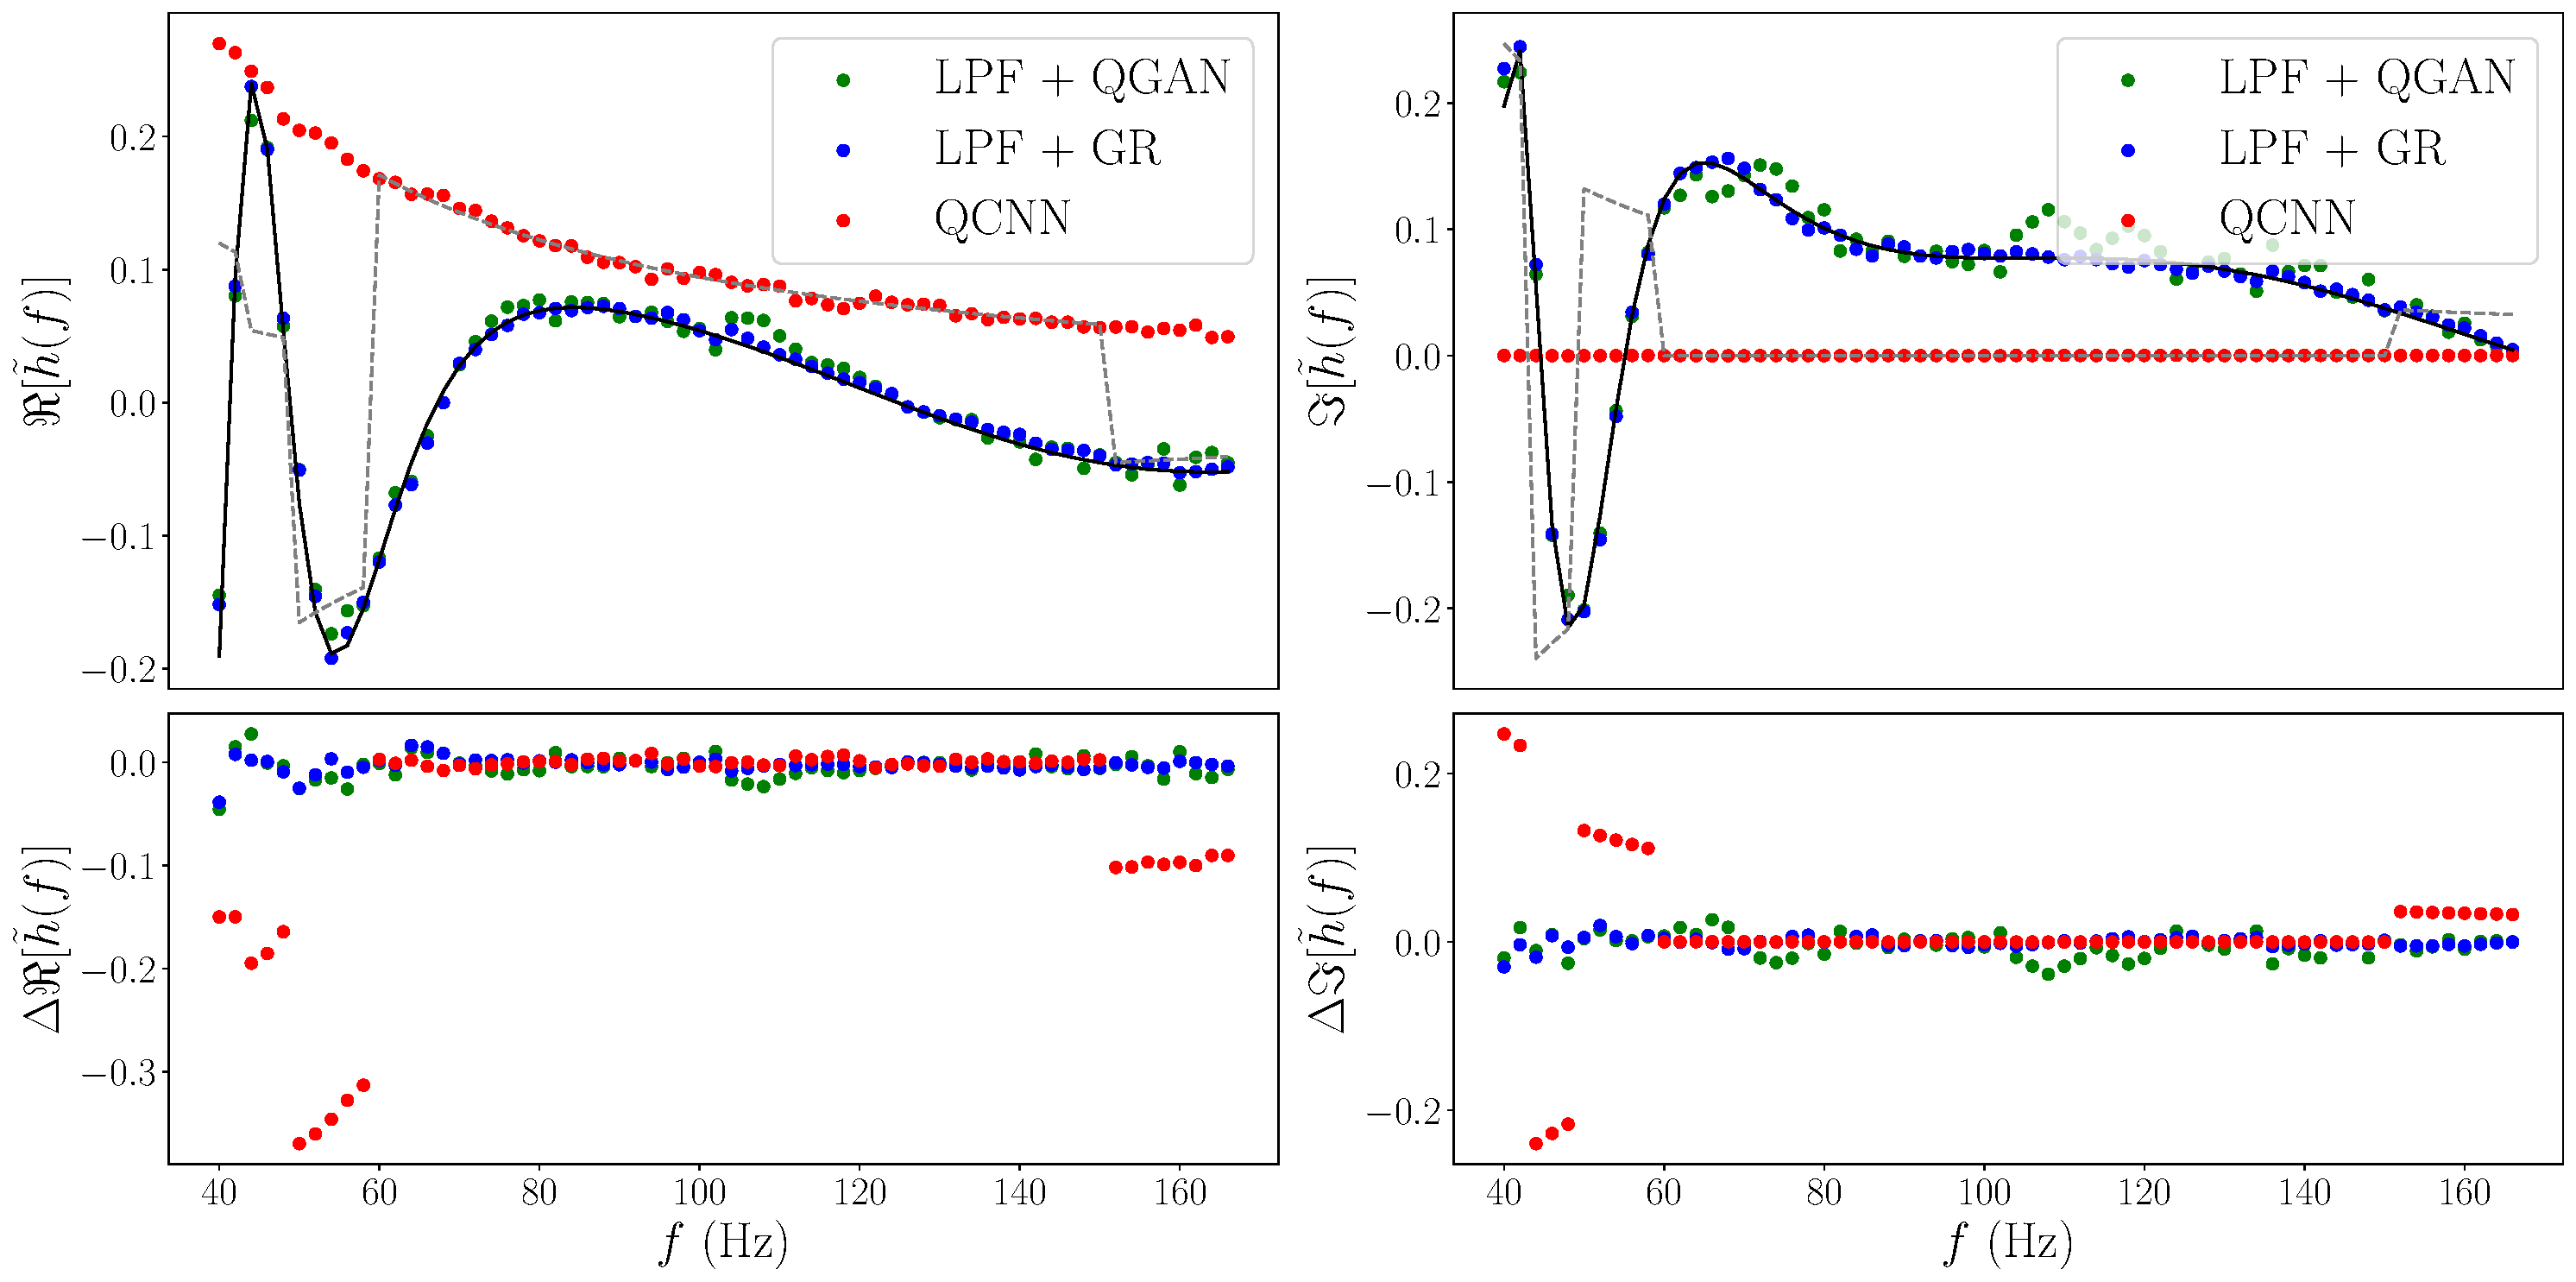
\includegraphics[width=\textwidth]{im/h_comp}
\caption{Encoding of $\boldsymbol{h}(f)$ as waveform $\tilde{h}(f)$ using different methods. Target in black; rounded target dashed in grey.}
\end{figure}
\end{frame}

\begin{frame}
\section{Next Steps}
\frametitle{Next Steps}
\begin{itemize}
\item more fully explore PQC parameter space ... (depth, epoch...)
\item look into barren plateau mitigation (layer-by-layer training....) => might help increase L/e
\end{itemize}
\end{frame}


\end{document}